%
% waerme.tex
%
% (c) 2018 Prof Dr Andreas Müller, Hochschule Rapperswil
%
\documentclass[tikz]{standalone}
\usepackage{times}
\usepackage{txfonts}
\usepackage[utf8]{inputenc}
\usepackage{graphics}
\usepackage{ifthen}
\usepackage{color}
\usetikzlibrary{arrows,intersections}
\usetikzlibrary{math}
\begin{document}

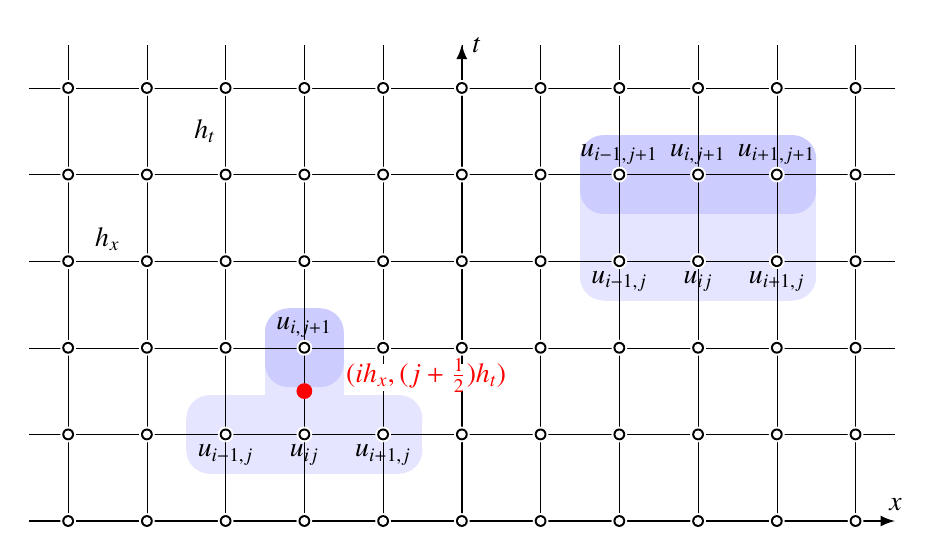
\begin{tikzpicture}[>=latex,thick]

\def\hx{1.0}
\def\hy{1.1}

\def\punkt#1#2{
        \fill[color=white] ({#1},{#2*\hy}) circle[radius=0.1];
        \fill              ({#1},{#2*\hy}) circle[radius=0.075];
        \fill[color=white] ({#1},{#2*\hy}) circle[radius=0.05];
}

\fill[color=blue!10] ({2*\hx-0.2},{3*\hy-0.2}) circle[radius=0.3];
\fill[color=blue!10] ({4*\hx+0.2},{3*\hy-0.2}) circle[radius=0.3];
\fill[color=blue!10] ({2*\hx-0.2},{4*\hy+0.2}) circle[radius=0.3];
\fill[color=blue!10] ({4*\hx+0.2},{4*\hy+0.2}) circle[radius=0.3];

\fill[color=blue!10] ({2*\hx-0.2},{3*\hy-0.5}) rectangle ({4*\hx+0.2},{4*\hy+0.5});
\fill[color=blue!10] ({2*\hx-0.5},{3*\hy-0.2}) rectangle ({4*\hx+0.5},{4*\hy+0.2});

\fill[color=blue!20] ({2*\hx-0.2},{4*\hy-0.2}) circle[radius=0.3];
\fill[color=blue!20] ({2*\hx-0.2},{4*\hy+0.2}) circle[radius=0.3];
\fill[color=blue!20] ({4*\hx+0.2},{4*\hy-0.2}) circle[radius=0.3];
\fill[color=blue!20] ({4*\hx+0.2},{4*\hy+0.2}) circle[radius=0.3];
\fill[color=blue!20] ({2*\hx-0.2},{4*\hy-0.5})
	rectangle ({4*\hx+0.2},{4*\hy+0.5});
\fill[color=blue!20] ({2*\hx-0.5},{4*\hy-0.2})
	rectangle ({4*\hx+0.5},{4*\hy+0.2});

\node at ({2*\hx},{3*\hy}) [below] {$u_{i-1,j}$};
\node at ({3*\hx},{3*\hy}) [below] {$u_{ij}$};
\node at ({4*\hx},{3*\hy}) [below] {$u_{i+1,j}$};

\node at ({2*\hx},{4*\hy}) [above] {$u_{i-1,j+1}$};
\node at ({3*\hx},{4*\hy}) [above] {$u_{i,j+1}$};
\node at ({4*\hx},{4*\hy}) [above] {$u_{i+1,j+1}$};

\fill[color=blue!10] ({-3*\hx-0.2},{1*\hy-0.2}) circle[radius=0.3];
\fill[color=blue!10] ({-3*\hx-0.2},{1*\hy+0.2}) circle[radius=0.3];
\fill[color=blue!10] ({-1*\hx+0.2},{1*\hy-0.2}) circle[radius=0.3];
\fill[color=blue!10] ({-1*\hx+0.2},{1*\hy+0.2}) circle[radius=0.3];
\fill[color=blue!10] ({-2*\hx-0.2},{2*\hy+0.2}) circle[radius=0.3];
\fill[color=blue!10] ({-2*\hx+0.2},{2*\hy+0.2}) circle[radius=0.3];

\fill[color=blue!10] ({-3*\hx-0.5},{1*\hy-0.2})
	rectangle ({-1*\hx+0.5},{1*\hy+0.2});
\fill[color=blue!10] ({-3*\hx-0.2},{1*\hy-0.5})
	rectangle ({-1*\hx+0.2},{1*\hy+0.5});
\fill[color=blue!10] ({-2*\hx-0.5},1) rectangle ({-2*\hx+0.5},{2*\hy+0.2});
\fill[color=blue!10] ({-2*\hx-0.2},1) rectangle ({-2*\hx+0.2},{2*\hy+0.5});

\fill[color=blue!20] ({-2*\hx-0.2},{2*\hy-0.2}) circle[radius=0.3];
\fill[color=blue!20] ({-2*\hx-0.2},{2*\hy+0.2}) circle[radius=0.3];
\fill[color=blue!20] ({-2*\hx+0.2},{2*\hy-0.2}) circle[radius=0.3];
\fill[color=blue!20] ({-2*\hx+0.2},{2*\hy+0.2}) circle[radius=0.3];
\fill[color=blue!20] ({-2*\hx-0.2},{2*\hy-0.5})
	rectangle ({-2*\hx+0.2},{2*\hy+0.5});
\fill[color=blue!20] ({-2*\hx-0.5},{2*\hy-0.2})
	rectangle ({-2*\hx+0.5},{2*\hy+0.2});

\node at ({-3*\hx},{1*\hy}) [below] {$u_{i-1,j}$};
\node at ({-2*\hx},{1*\hy}) [below] {$u_{ij}$};
\node at ({-1*\hx},{1*\hy}) [below] {$u_{i+1,j}$};
\node at ({-2*\hx},{2*\hy}) [above] {$u_{i,j+1}$};

\draw[->] (-5.5,0)--(5.5,0) coordinate[label=$x$];
\draw[->] (0,0)--(0,{5.5*\hy}) coordinate[label={right:$t$}];

\foreach \y in {1,2,...,5}{
	\draw[line width=0.1pt] (-5.5,{\y*\hy})--(5.5,{\y*\hy});
}
\foreach \x in {-5,-4,...,5}{
	\draw[line width=0.1pt] ({\x*\hx},0)--({\x*\hx},{5.5*\hy});
	\foreach \y in {0,1,...,5}{
		\punkt{\x}{\y}
	}
}

\node at ({-4.5*\hx},{3*\hy}) [above] {$h_x$};
\node at ({-3*\hx},{4.5*\hy}) [left] {$h_t$};

\fill[color=red] ({-2*\hx},{1.5*\hy}) circle[radius=0.1];
\fill[color=white] ({-1.5*\hx},{1.5*\hy}) rectangle ({0.5*\hx},{2*\hy-0.2});
\node[color=red] at ({-2*\hx+0.4},{1.5*\hy+0.2}) [right] {$(ih_x,(j+\frac12)h_t)$};

\end{tikzpicture}

\end{document}
